\documentclass[10pt]{article}
\usepackage[margin=0.72in]{geometry}
\usepackage{graphicx}
\usepackage{array}
\usepackage[T1]{fontenc}
\pagestyle{empty}
\begin{document}
\begin{center}
{\Large\bfseries Exact experiment ID pointers in formal targets}\\[4pt]
{\small crypto-autoresearcher, 2026-10-27; source commit
\texttt{351c9c021c7be044ade54dc7e352b33d3a772244}}
\end{center}

\noindent\textbf{Question.} Which existing experiment-directory IDs occur as
exact tokens in a registered formal target, its declared text source, or its
Lean theorem source? This is a syntactic inventory, not a theorem or run
review.

\begin{center}
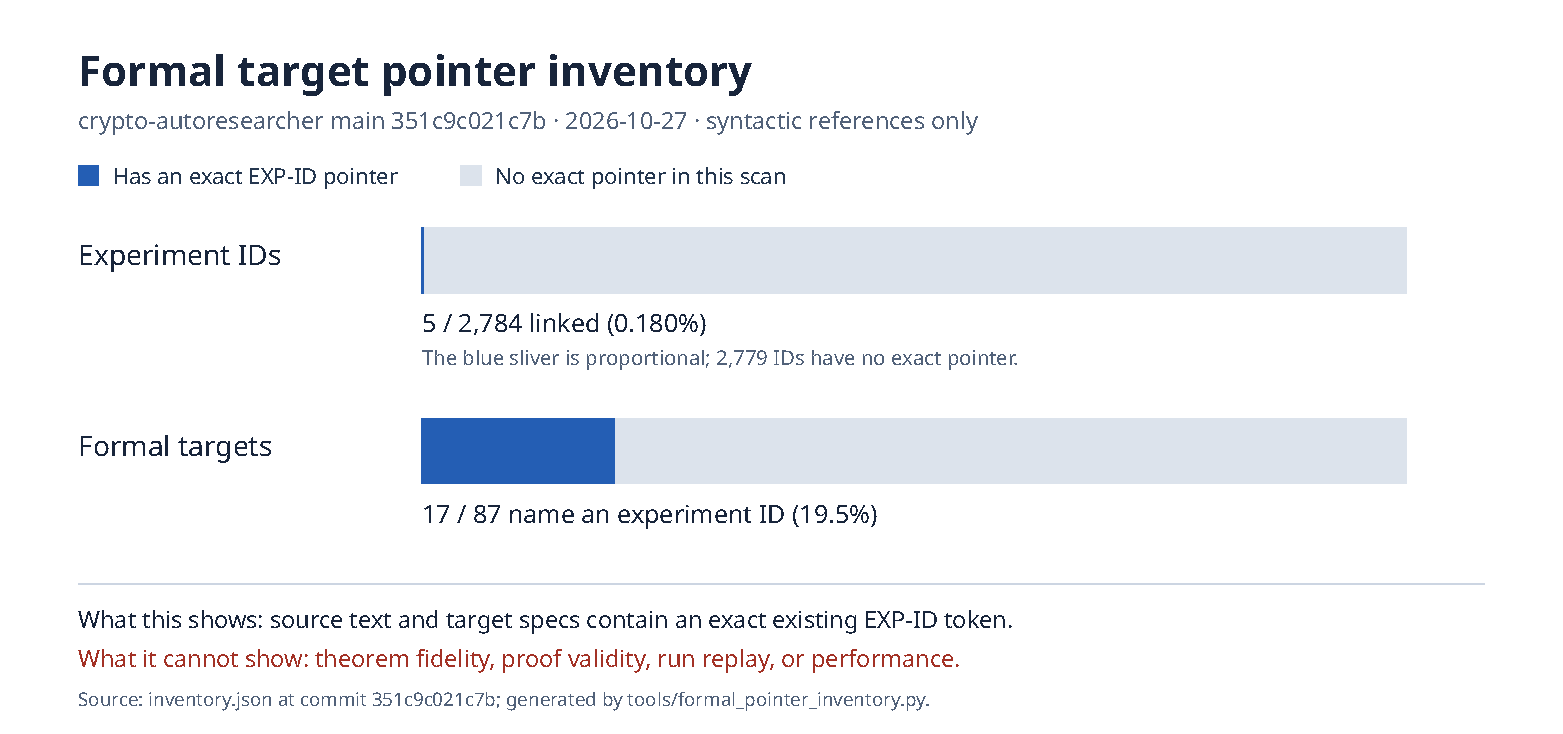
\includegraphics[width=0.98\linewidth]{coverage-figure.pdf}
\end{center}

\noindent\textbf{Method.} The repository tool reads immutable Git objects,
enumerates tracked \texttt{EXP-*} directories and all 87 registered target
YAMLs, then scans target and named text-source bytes for exact existing IDs.
No source exceeded the 1~MB scan limit. The machine-readable
\texttt{inventory.json} binds the tree hashes, all IDs, and each witness path.

\medskip
\noindent\textbf{Result.} Five of 2,784 experiment IDs have an exact pointer
in 17 of 87 registered targets. The five are BINSTD-8bdf86, FROB-91ee9c,
FROB-b8cf21, GFPN-05ff43, and NCP-001 (all prefixed \texttt{EXP-}).
NCP-001 occurs in the declared NCP theory note and was absent from the
earlier local diagnostic. Its pointer does not certify the full experiment
claim.

\medskip
\noindent\textbf{Boundary.} A present pointer does not establish Lean
validity, semantic fidelity, archived execution, or a performance/security
claim. An absent pointer does not establish that no relevant theorem exists.
This report covers the committed autoresearcher \texttt{main} tree only;
\texttt{crypto}, \texttt{cryptanalysis}, open PRs, and uncommitted work need
separate inventories. No research decision or status changed.

\medskip
\noindent\textbf{Reproduction.} Run the command below from the repository
root. The complete method, limits, and next checks are in \texttt{REPORT.md}.
\begin{verbatim}
python3 tools/formal_pointer_inventory.py \
  --repo . \
  --revision 351c9c021c7be044ade54dc7e352b33d3a772244 \
  --out /tmp/pointers.json
\end{verbatim}
\end{document}
